\chapter{Concepte teoretice despre învățare automată}

\section{Recunoașterea vorbirii}
Pentru a putea recunoaște vorbirea dintr-un videoclip, am ales să folosesc arhitectura
\textit{wav2vec 2.0} \cite{wav2vec2} dezvoltată de Facebook AI Research. Am folosit 
atât modelul \textit{facebook/wav2vec2-base-960h} antrenat pe setul de date 
\textit{LibriSpeech} \cite{librispeech}, cât și modelul preantrenat
\textit{facebook/wav2vec2-base} pe care le-am antrenat pe seturile
de date \textit{Mini LibriSpeech} (subset din LibriSpeech) și
\textit{Common Voice Delta Segment 16.1} (subset din Common Voice) \cite{commonvoice}.
\par

\subsection{Semnalul audio}
\label{subsec:semnal-audio}
Înainte de a intra în detalii despre modelele folosite, este important să înțelegem în 
ce constă semnalul audio, cum este reprezentat în memorie și cum este procesat.

\par
Definim un convertor analog-digital ca fiind un dispozitiv care transformă semnalul recepționat 
de la microfon (variații în presiunea aerului/unde sonore) într-un semnal digital.
Practic, convertește semnalul analogic continuu într-un
semnal digital discret care poate fi stocat și procesat de un calculator. Acest proces implică
conceptul de cuantizare și introduce o eroare de cuantizare care depinde de rezoluția convertorului.
În acest sens, convertorul analog-digital convertește periodic semnalul analogic, eșantionând semnalul
la intervale de timp egale.
\par
Perioada de timp dintre două eșantioane consecutive este cunoscută sub numele de \textbf{frecvență de eșantionare}
și este măsurată în Hz. Cu cât frecvența de eșantionare este mai mare, cu atât semnalul digital este mai apropiat
de semnalul analogic original. Această frecvență măsoară numărul de sample-uri pe secundă.
\par
Conceptul de \textbf{rezoluție} indică numărul de valori discrete distincte pe care le poate 
reprezenta un convertor analog-digital. Cu cât rezoluția este mai mare, cu atât semnalul digital
este mai apropiat de semnalul analogic original.
\par
De exemplu, un convertor analog-digital cu o rezoluție de 8 biți poate encoda un semnal analogic
în $2^8 = 256$ de valori discrete. Figura de mai jos ilustrează procesul de conversie analog-digital
și digital-analog. (Fig. \ref{fig:conversion-ad-da})

\begin{figure}[h]
    \centering
    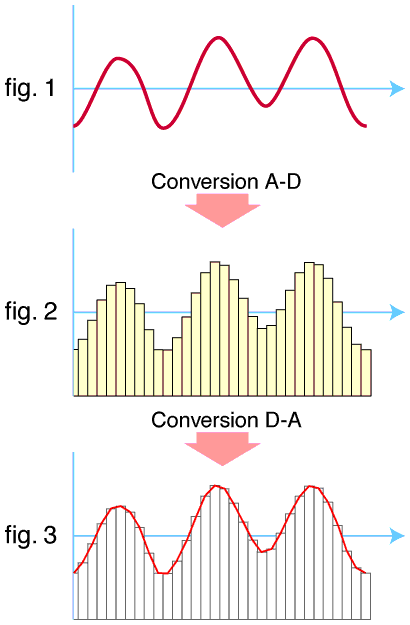
\includegraphics[width=0.5\textwidth]{Conversion_AD_DA.png}
    \caption{Procesul de conversie analog-digital și digital-analog\protect\footnotemark[1]}
    \label{fig:conversion-ad-da}
\end{figure}
\footnotetext[1]{Imagine preluată de pe Wikipedia la adresa: \url{https://en.wikipedia.org/wiki/Analog-to-digital_converter}}

\par
Acum că am definit cum sunt interpretate semnalele audio, putem să trecem la procesarea acestora.
Definim ce semnifică valorile obținute (Fig. \ref{fig:pcm}):

\begin{itemize}
    \item \textbf{Amplitudinea}: reprezintă presiunea undelor sonore măsurată la un moment de timp.
    Cu cât amplitudinea este mai mare, cu atât sunetul este mai puternic.
    \item \textbf{Ampitudinea zero}: valoarea 0 reprezintă linia de bază a semnalului audio, punctul
    principal de referință după care se măsoară amplitudinea.
    \item \textbf{Valori pozitive și negative}: valorile sunt reprezentate în formatul PCM (\textit{Pulse Code Modulation}),
    unde valorile pozitive sunt reprezentate de valori între 0 și 1, iar valorile negative sunt reprezentate
    de valori între 0 și -1.
\end{itemize}

\begin{figure}[h]
    \centering
    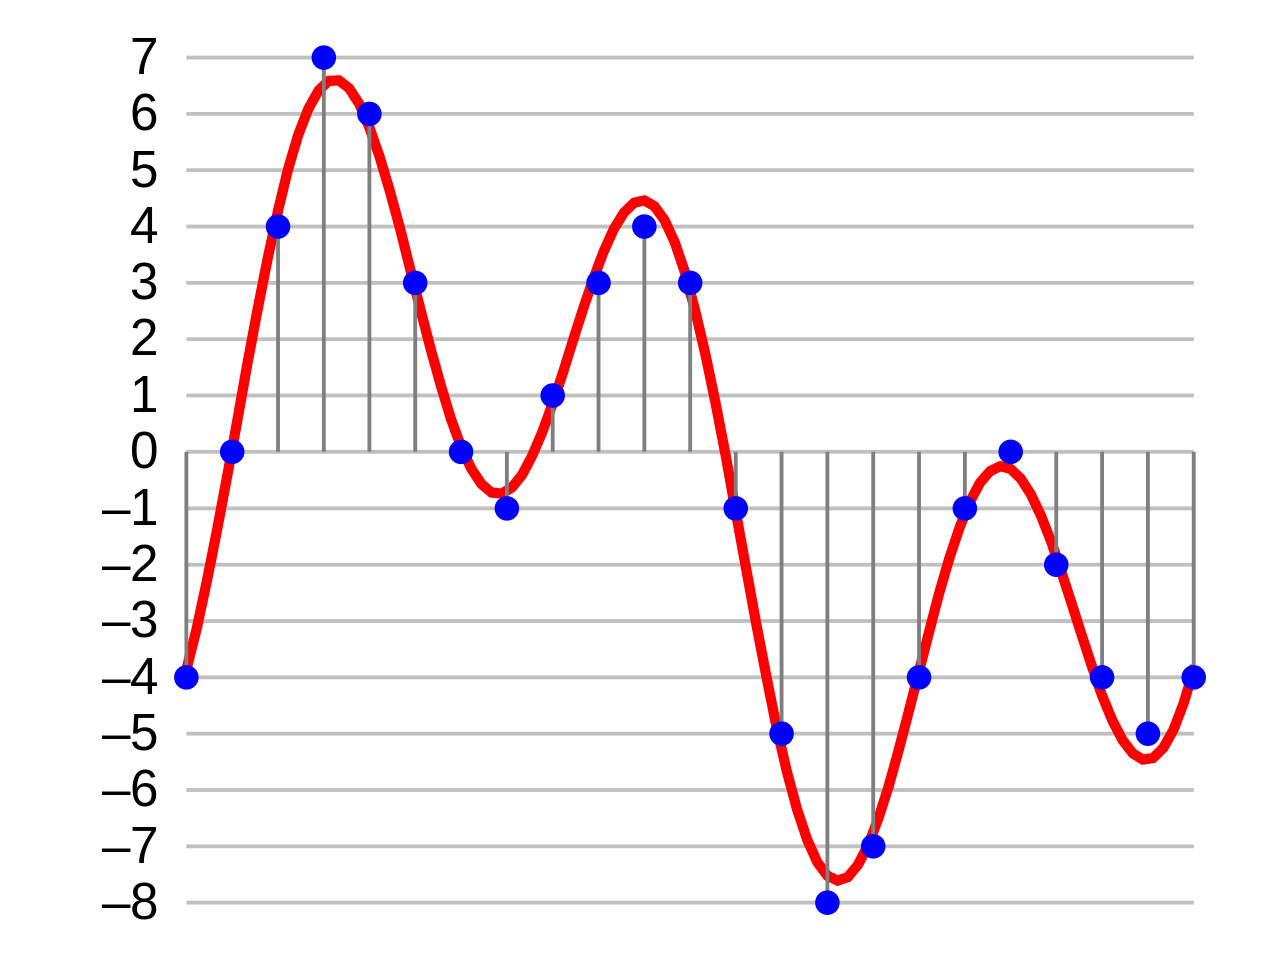
\includegraphics[width=0.4\textwidth]{PCM.png}
    \caption{Reprezentarea semnalului audio în format PCM\protect\footnotemark[1]}
    \label{fig:pcm}
\end{figure}

\par
De aici încolo vom lucra cu semnalul digital în Python folosind librăriile \textit{soundfile},
\textit{librosa} și \textit{numpy} pentru a procesa secvențele audio.
\footnotetext[1]{Imagine preluată de pe Wikipedia la adresa: \url{https://en.wikipedia.org/wiki/Audio_bit_depth}}
\footnotetext[2]{Imagine preluată de pe site-ul lui Jonathan Bgn, ``Illustrated Wav2Vec 2.0'', disponibil la: \url{https://jonathanbgn.com/2021/09/30/illustrated-wav2vec-2.html}.}
\vspace{-1em}
\subsection{Arhitectura modelului}
Modelul \textit{wav2vec 2.0} este un model de învățare profundă alcătuit din 4
componente principale: \textbf{Codificator de Caracteristici Latente} 
(\textit{Latent Feature Encoder}), reprezentat de o \textit{Rețea Neuronală Convoluțională},
\textbf{Rețea pentru Context} (\textit{Context Network}), constă în partea de Encodare
a Transformer-ului, \textbf{Modulul de Cuantizare} (\textit{Quantization Module}),
aplică funcția \textit{Gumbel Softmax} și \textbf{Pierderea Contrastivă}. (Fig. \ref{fig:wav2vec2-architecture})

\begin{figure}[h]
    \centering
    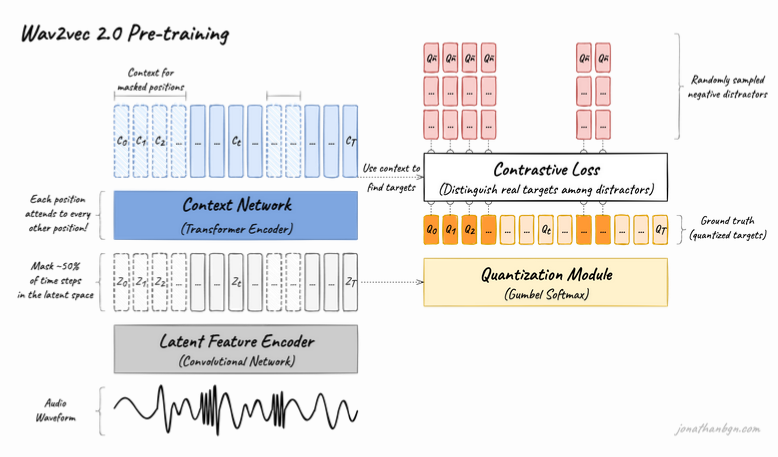
\includegraphics[width=1\textwidth]{wav2vec2-architecture.png}
    \caption{Arhitectura modelului \textit{wav2vec 2.0} \protect\footnotemark[2]}
    \label{fig:wav2vec2-architecture}
\end{figure}

\subsubsection{Codificator de Caracteristici Latente}
\textbf{Codificatorul de caracteristici latente} (\textit{Latent Feature Encoder}) este prima parte a modelului
\textit{wav2vec 2.0} și se ocupă cu prelucrarea semnalului audio (explicat anterior în secțiunea \ref{subsec:semnal-audio}).
Astfel, Codificatorul de Caracteristici Latente procesează semnalul audio din forma lui inițială folosind o 
normalizare de medie 0 și deviație standard 1. Apoi, continuă cu 7 blocuri convoluționale, fiecare alcătuit
din convoluții 1-dimensionale, normalizare la nivel de strat și activări GELU (\textit{Gaussian Error Linear Unit}).
\par
Dimensiunea canalelor, a filtrului și a lungimii pasului sunt prezentate în figura de mai jos
(Fig. \ref{fig:latent-feature-encoder}). În această etapă, modelul încearcă să înțeleagă legătura dintre
valorile apropiate ale semnalului audio și să să extragă caracteristici latente care vor fi folosite ulterior. Arhitectura
blocurilor convoluționale este structurată astfel:
\begin{itemize}
    \item \textbf{Blocul 1}: dimensiunea filtrului 10, lungimea pasului 5, canale 512
    \item \textbf{Blocurile 2-5}: dimensiunea filtrului 3, lungimea pasului 2, canale 512
    \item \textbf{Blocurile 6-7}: dimensiunea filtrului 2, lungimea pasului 2, canale 512
\end{itemize}


\vspace{-0.5em}
\begin{figure}[h]
    \centering
    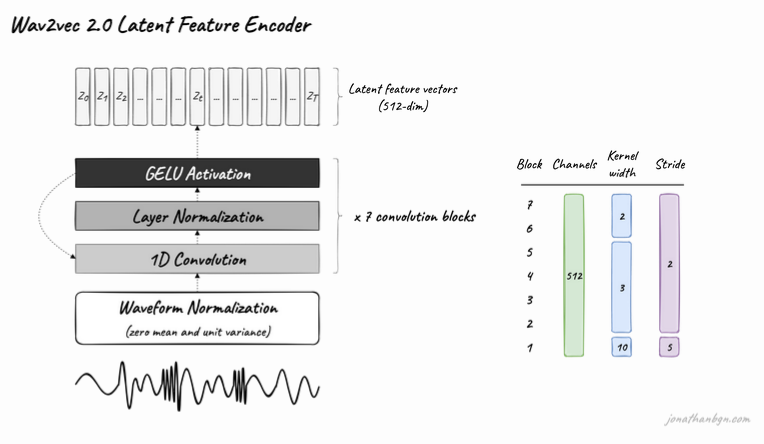
\includegraphics[width=1\textwidth]{wav2vec2-feature-encoder.png}
    \caption{Arhitectura componentei \textit{Latent Feature Encoder} \protect\footnotemark[1]}
    \label{fig:latent-feature-encoder}
\end{figure}
\vspace{-0.5em}
\par
Se observă cum primul bloc convoluțional are dimensiunea filtrului 10 și lungimea pasului 5,
fiind cele mai mari valori din cele 7 blocuri. Intuitiv, acest bloc încearcă să acopere o porțiune
mai mare din semnalul audio, în timp ce blocurile următoare (cu dimensiuni mai mici) încearcă să
înțeleagă detalii mai fine din semnalul audio. în
\footnotetext[1]{Imagine preluată de pe site-ul lui Jonathan Bgn, ``Illustrated Wav2Vec 2.0'', disponibil la: \url{https://jonathanbgn.com/2021/09/30/illustrated-wav2vec-2.html}.}

\subsubsection{Rețea pentru Context}
\vspace{1em}
Componenta \textbf{Rețea pentru context} (\textit{Context Network}) reprezintă inovația adusă de modelul
\textit{wav2vec 2.0} față de predecesorul său \textit{wav2vec} deoarece folosește un codificator de tip
\textit{Transformer} care oferă o reprezentare contextuală mult mai bună decât codificatorul convoluțional
folosit anterior.
\par
Asfel, caracteristicile extrase de componenta \textbf{Codificator de Caracteristici Latente} sunt 
proiectate într-un spațiu latent de dimensiune 768 pentru modelul \textit{BASE}, respectiv 1024 pentru modelul
\textit{LARGE} pentru a putea fi procesate de rețeaua de tip \textit{Transformer}. 
\par
Un alt aspect important, înainte de a trece prin rețeaua de tip \textit{Transformer}, îl reprezintă
\textit{encodarea pozițională} a caracteristicilor latente. Această encodare pozițională adaugă
informații despre poziția relativă a caracteristicilor la nivel de secvență, corelând astfel
caracteristicile cu poziția lor în secvența audio.
\par
În final, caracteristicile sunt trecute prin codificatorul de tip \textit{Transformer} care,
prin \textit{mecanismul de atenție}, învață legături între caracteristici și poziția lor în secvență,
oferind o reprezentare contextuală cât mai bună a semnalului audio. 

\vspace{2em}
\begin{figure}[h]
    \centering
    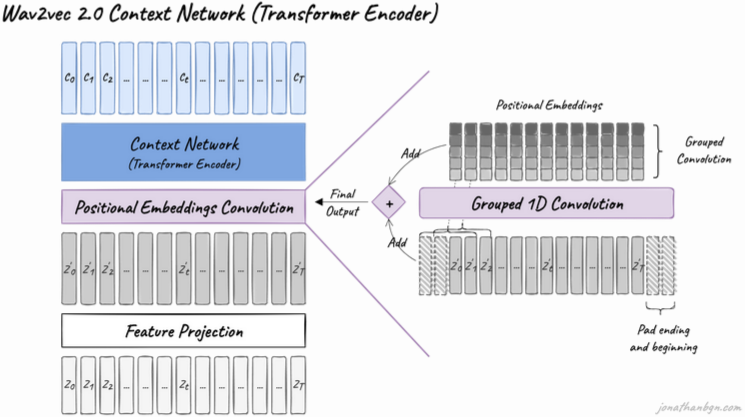
\includegraphics[width=1\textwidth]{wav2vec2-context-network.png}
    \caption{Arhitectura componentei \textit{Context Network} \protect\footnotemark[1]}
    \label{fig:wav2vec2-context-network}
\end{figure}
\vspace{1em}
\footnotetext[1]{Imagine preluată de pe site-ul lui Jonathan Bgn, ``Illustrated Wav2Vec 2.0'', disponibil la: \url{https://jonathanbgn.com/2021/09/30/illustrated-wav2vec-2.html}.}

\subsubsection{Modulul de cuantizare}
\vspace{1em}
Din cauza naturii continue a semnalului audio, modelul \textit{wav2vec 2.0} nu poate folosi în mod direct
un vocabular discret de simboluri, așa cum întâlnim în limbajul scris. Astfel, autorii modelului propun
conceptul de \textbf{codebook} alcătuit \textbf{codewords} pentru a discretiza semnalul audio. Intuitiv,
ne putem gândi la \textit{codebook} ca la un vocabular de sunete fonetice reprezentative pentru semnalul
audio. Deoarece un semnalul audio poate conține mai multe sunete fonetice, autorii propun folosirea
a G \textit{codebooks} fiecare cu câte V \textit{codewords} creând astfel o matrice denumită \textit{matricea
de cuantizare}.
\par
După înmulțirea caracteristicilor din spațiul latent cu matricea de cuantizare, se aplică funcția
\textbf{Gumbel Softmax} peste logits și se obțin astfel vectori care conțin valoarea 1 pe poziția
corespunzătoare sunetului fonetic și 0 pe restul pozițiilor. Spre deosebire de funcția \textit{Softmax},
funcția \textit{Gumbel Softmax} adaugă zgomot de medie 0 și deviație standard 1, zgomot reglat cu 
ajutorul temperaturii, care ajută modelul să exploreze mai multe sunete fonetice în timpul antrenării.
De asemnea, funcția \textit{Gumbel Softmax} este o funcție diferențiabilă care permite antrenarea modelului
prin tehnica de \textbf{coborârii pe gradient}.
\par
Vectorii menționați anterior indică poziția sunetului fonetic în \textit{codebook} și sunt înmulțiți
apoi cu o matrice de proiecție pentru a redimensionarea caracteristicile la dimensiunea ieșirilor
codificatorului de tip Transformer.
\footnotetext[1]{Imaginile au fost preluate de pe site-ul lui Jonathan Bgn, ``Illustrated Wav2Vec 2.0'', disponibil la: \url{https://jonathanbgn.com/2021/09/30/illustrated-wav2vec-2.html}.}

\vspace{1.5em}
\begin{figure}[h]
    \centering
    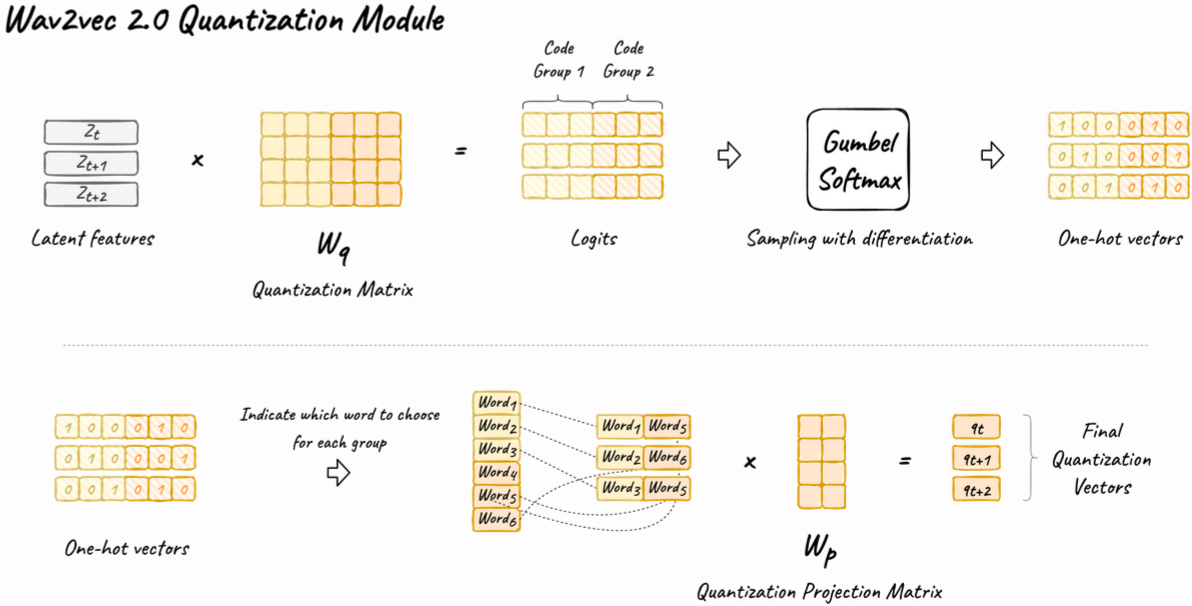
\includegraphics[width=1\textwidth]{wav2vec2-quantization-module.png}
    \caption{Arhitectura componentei \textit{Quantization Module} \protect\footnotemark[1]}
    \label{fig:wav2vec2-quantization-module}
\end{figure}
\vspace{1em}

\subsubsection{Pierdere contrastivă}
În special pentru partea de preantrenare a modelului, în care scopul principal este înțelegerea
dependențelor între caracteristicile latente ale semnalului audio, autorii propun folosirea unei
funcții de pierdere contrastivă. 
\par
Astfel, pentru a forța modelul să învețe reprezentări semantice, se folosește o mască care ascunde
$\sim$50\% din vectorii proiectați din spațiul latent înainte să fie trecuți prin \textbf{Rețeaua pentru Context}.
În procesul de învățare, vectorii mascați vor fi înlocuiți apoi cu reprezentările învățate de model.

\par
Pentru fiecare poziție mascată, se aleg uniform aleator 100 de exemple negative de la alte poziții
și se compară \textbf{similaritatea cosinus} între vectorul proiectat și vectorii aleși.
Astfel, funcția de pierdere contrastivă încurajează similaritatea cu exemplele \textit{adevărat pozitive}
și penalizează similaritatea cu exemplele \textit{negative}.
\par
De asemenea, în timpul preantrenării, se folosește și o funcție de pierdere pentru diversitatea \textit{codewords}, numită
\textit{Diversity Loss}, care maximizează entropia distribuției \textit{Gumbel-Softmax}. Această funcție
impune modelului să exploreze mai multe sunete fonetice în timpul antrenării și previne blocarea pe un
subset de sunete.

\vspace{1em}
\begin{figure}[h]
    \centering 
    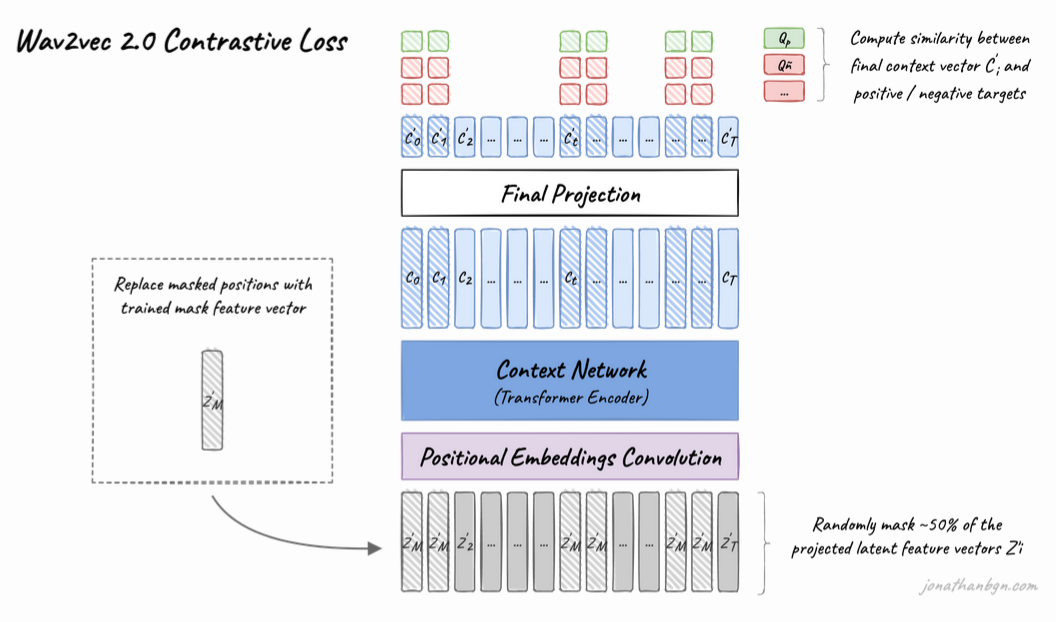
\includegraphics[width=1\textwidth]{wav2vec2-contrastive-loss.png}
    \caption{Arhitectura componentei \textit{Contrastive Loss} \protect\footnotemark[1]}
    \label{fig:wav2vec2-contrastive-loss}
\end{figure}
\vspace{1em}

\footnotetext[1]{Imaginile au fost preluate de pe site-ul lui Jonathan Bgn, ``Illustrated Wav2Vec 2.0'', disponibil la: \url{https://jonathanbgn.com/2021/09/30/illustrated-wav2vec-2.html}.}

\subsection{Setul de date}
Modelul oficial a fost preantrenat pe setul de date \textit{LibriSpeech}, iar eu am continuat
antrenarea pe seturile de date \textit{Mini LibriSpeech} și \textit{Common Voice Delta Segment 16.1}.

\subsubsection{Mini-LibriSpeech}
\textit{Mini LibriSpeech} este un subset al setului de date \textit{LibriSpeech} care conține 
aproximativ 2 ore de înregistrări audio la o frecvență de eșantionare de 16 kHz. În medie,
fiecare înregistrare are o durată de 6.72 secunde, cel mai lung audio având o durată de 31.5 secunde.

\subsubsection{Common Voice Delta Segment 16.1}
\textit{Common Voice Delta Segment 16.1} este un subset al setului de date \textit{Common Voice}
care conține aproximativ 2 ore de înregistrări audio la o frecvență de eșantionare de 48 kHz.
A fost nevoie să reducem frecvența de eșantionare la 16 kHz pentru a putea folosi aceste date la
antrenarea modelului. În medie, fiecare înregistrare are o durată de 5.63 secunde, cel mai lung
audio având o durată de 10.47 secunde.

\begin{figure}[h]
    \centering
    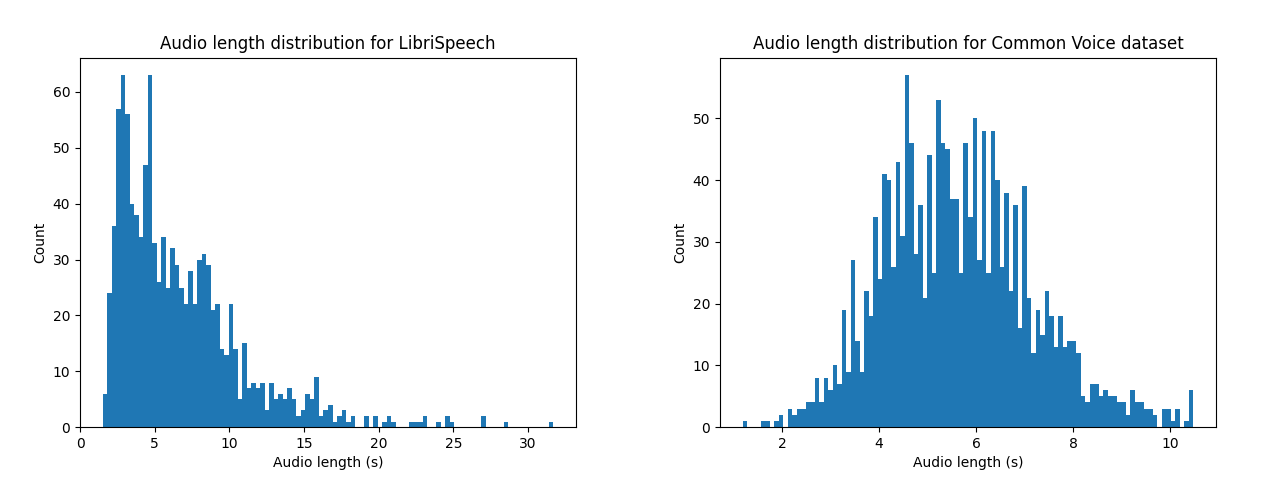
\includegraphics[width=1\textwidth]{length_distribution.png}
    \caption{Distribuția duratelor secvențelor audio din seturile de date \textit{Mini LibriSpeech} și \textit{Common Voice Delta Segment 16.1}}
    \label{fig:length-distribution}
\end{figure}

\subsubsection{Concluzie}
Menționăm aceste detalii deoarece pentru generarea subtitrărilor vom avea nevoie de secvențe audio
mult mai lungi decât cele folosite pentru antrenare, care nu ar încăpea în memorie. Astfel, va trebui
să folosim o tehnică de segmentare a secvențelor audio în bucăți mai mici pentru a putea fi procesate.
Mai multe detalii despre această tehnică vor fi prezentate în secțiunea \textit{Subtitrări}. \ref{subsec:subtitles}

\subsection{Antrenarea modelului}
Pentru antrenarea modelului am folosit limbajul de programare \textit{Python} și biblioteca \textit{Hugging Face}
care pune la dispoziție o serie de librării precum \textit{transformers} și \textit{datasets}.
\par
Hiperparametrii folosiți pentru antrenarea modelului sunt:
\begin{itemize}
    \item \textbf{Rata de învățare} - pentru a controla cât de mult se vor actualiza ponderile în timpul
    antrenării, poate fi gândit ca lungimea pasului în direcția gradientului
    \item \textbf{Declinul ponderilor} - pentru a menține sub control creșterea ponderilor în timpul antrenării
    și pentru a evita gradienții instabili
    \item \textbf{Pași de încălzire} - pentru a controla cum se modifică rata de învățare în prima parte 
    a antrenării
    \item \textbf{Dimensiunea lotului} - câte exemple se procesează în același timp
\end{itemize}

\vspace{0.5em}

\begin{table}[h]
    \centering
    \caption{Hiperparametrii folosiți pentru antrenarea modelului \textit{wav2vec2}}
    \label{tab:wav2vec2-hyperparameters}
    \begin{tabular}{@{}lp{2cm}@{}} % Adjusting column width
    \toprule % Top horizontal line
    \textbf{Hiperparametru} & \textbf{Valoare} \\
    \midrule % Middle horizontal line
    Rata de învățare & $1 \times 10^{-4}$ \\
    Declinul ponderilor & 0.005 \\
    Pași de încălzire & 1000 \\
    Dimnesiunea lotului & 4 \\
    \bottomrule % Bottom horizontal line
    \end{tabular}
\end{table}

\par
Am antrenat modelul pe seturile de date \textit{Mini LibriSpeech} și \textit{Common Voice Delta Segment 16.1}
pe o placă grafică \textit{NVIDIA Tesla V100} pusă la dispoziție de \textit{Google Colab}. Am salvat starea modelului
la fiecare 500 de pași pentru a putea monitoriza evoluția modelului. Rezultatele obținute la fiecare punct de control
\textit{facebook/wav2vec2-base} sunt prezentate în cele două tabele de mai jos.


% \begin{figure}[h]
%     \centering
%     \begin{minipage}{.5\textwidth}
%         \centering
%         \captionsetup{justification=centering} 
%         \captionof{table}{Mini LibriSpeech}
%         \label{tab:model-checkpoints1}
%         \begin{tabular}{cccc}
%         \toprule
%         \textbf{Step} & \textbf{Train loss} & \textbf{Val loss} & \textbf{wer(\%)} \\
%         \midrule
%         500  & 3.840 & 3.099 & 1.000 \\
%         1000 & 1.202 & 0.586 & 0.361 \\
%         1500 & 0.360 & 0.352 & 0.265 \\
%         2000 & 0.231 & 0.333 & 0.222 \\
%         2500 & 0.163 & 0.357 & 0.230 \\
%         3000 & 0.136 & 0.331 & 0.199 \\
%         3500 & 0.114 & 0.369 & 0.205 \\
%         4000 & 0.104 & 0.348 & 0.203 \\
%         4500 & 0.094 & 0.335 & 0.177 \\
%         5000 & 0.083 & 0.284 & 0.165 \\
%         5500 & 0.078 & 0.332 & 0.165 \\
%         6000 & 0.072 & 0.356 & 0.174 \\
%         6500 & 0.069 & 0.393 & 0.165 \\
%         7000 & 0.066 & 0.380 & 0.181 \\
%         \bottomrule
%         \end{tabular}
%     \end{minipage}%
%     \begin{minipage}{.5\textwidth}
%         \centering
%         \captionof{table}{Common Voice Delta 16.1}
%         \label{tab:model-checkpoints2}
%         \begin{tabular}{cccc}
%         \toprule
%         \textbf{Step} & \textbf{Train loss} & \textbf{Val loss} & \textbf{wer(\%)} \\
%         \midrule
%         500  & 3.919 & 3.236 & 1.000 \\
%         1000 & 1.287 & 0.570 & 0.398 \\
%         1500 & 0.368 & 0.400 & 0.261 \\
%         2000 & 0.226 & 0.371 & 0.252 \\
%         2500 & 0.166 & 0.402 & 0.239 \\
%         3000 & 0.136 & 0.475 & 0.233 \\
%         3500 & 0.116 & 0.445 & 0.201 \\
%         4000 & 0.097 & 0.448 & 0.196 \\
%         4500 & 0.096 & 0.404 & 0.190 \\
%         5000 & 0.079 & 0.459 & 0.182 \\
%         5500 & 0.080 & 0.400 & 0.182 \\
%         6000 & 0.069 & 0.445 & 0.182 \\
%         6500 & 0.073 & 0.421 & 0.179 \\
%         7000 & 0.064 & 0.440 & 0.182 \\
%         \bottomrule
%         \end{tabular}
%     \end{minipage}
% \end{figure}
    
\begin{figure}[h]
    \centering
    \begin{minipage}{.5\textwidth}
        \centering
        \captionsetup{justification=centering} 
        \captionof{table}{\textit{Mini LibriSpeech}}
        \label{tab:model-checkpoints1}
        \begin{tabular}{ccc}
        \toprule
        \textbf{Pas} & \textbf{Antrenare} & \textbf{Validare} \\
        \midrule
        500  & 3.840 & 3.099 \\
        1000 & 1.202 & 0.586 \\
        1500 & 0.360 & 0.352 \\
        2000 & 0.231 & 0.333 \\
        2500 & 0.163 & 0.357 \\
        3000 & 0.136 & 0.331 \\
        3500 & 0.114 & 0.369 \\
        4000 & 0.104 & 0.348 \\
        4500 & 0.094 & 0.335 \\
        5000 & 0.083 & 0.284 \\
        5500 & 0.078 & 0.332 \\
        6000 & 0.072 & 0.356 \\
        6500 & 0.069 & 0.393 \\
        7000 & 0.066 & 0.380 \\
        \bottomrule
        \end{tabular}
    \end{minipage}%
    \begin{minipage}{.5\textwidth}
        \centering
        \captionof{table}{\textit{Common Voice Delta 16.1}}
        \label{tab:model-checkpoints2}
        \begin{tabular}{ccc}
        \toprule
        \textbf{Pas} & \textbf{Antrenare} & \textbf{Validare} \\
        \midrule
        500  & 3.919 & 3.236 \\
        1000 & 1.287 & 0.570 \\
        1500 & 0.368 & 0.400 \\
        2000 & 0.226 & 0.371 \\
        2500 & 0.166 & 0.402 \\
        3000 & 0.136 & 0.475 \\
        3500 & 0.116 & 0.445 \\
        4000 & 0.097 & 0.448 \\
        4500 & 0.096 & 0.404 \\
        5000 & 0.079 & 0.459 \\
        5500 & 0.080 & 0.400 \\
        6000 & 0.069 & 0.445 \\
        6500 & 0.073 & 0.421 \\
        7000 & 0.064 & 0.440 \\
        \bottomrule
        \end{tabular}
    \end{minipage}
\end{figure}

\subsubsection{Notă}
Se observă că modelul a început să învețe destul de repede, scăzând pierderea de antrenare
de la 3.840 la 0.066, respectiv de la 3.919 la 0.064 în doar 7000 de pași. Urmărind graficul,
se observă fenomenul de \textit{overfitting} care apare în jurul pașilor 5000-6000, motiv
pentru care am ales să opresc antrenarea la 7000 de pași și sa folosesc modelul de
la pasul 5000, respectiv 5500.


% CITESTE INAINTE SA CONTINUI SA SCRII
% wer pare ca nu arata valorile corecte la antrenare
% ai testat in scriptul test.py modelul normal si modelul cu language model
% si ai obtinut valori corecte pentru wer

% - explica cum merge n-gram language model
% - arata imbunatatirea (ruleaza script ul test.py)
% - eventual fa discutie si despre fix spelling

\subsection{Îmbunătățire cu un model de limbaj}
Pentru a îmbunătăți recunoașterea vorbirii, am folosit un un model de limbaj bazat pe n-grame care 
mărește performanța modelului de la \textbf{wer 4.2\%}  la \textbf{wer 2.9\%}, aducând
o îmbunătățire de \textbf{1.3\%}.

\subsubsection{Model de limbaj bazat pe n-grame}
Un un model de limbaj bazat pe n-grame este un model statistic care estimează, în cazul nostru, probabilitatea
apariției unui caracter având în vedere cele n-1 caractere anterioare. Modelul se bazează pe
ipoteza \textbf{Markov de ordinul n}, conform căreia putem aproxima probabilitatea apariției unui caracter
folosind doar ultimele n caractere. Formula de mai jos ilustrează această idee:

\begin{equation}
    P(w_1, w_2, \ldots, w_n) = \prod_{i=1}^{m} P(w_i | w_{1}, w_{2}, \ldots, w_{i-1}) \approx \prod_{i=1}^{m} P(w_i | w_{i-(n-1)}, \ldots, w_{i-1})
\end{equation}
\vspace{1em}

\par
Am folosit un context de 5 caractere și am antrenat modelul pe
setul de date \textit{Helsinki-NLP/europarl} \cite{tiedemann-2012-parallel} deoarece conține și
texte în limba engleză și putem avea certitudinea că textele sunt corecte din punct de vedere
gramatical. Cu ajutorul librăriei \textit{KenLM} \cite{heafield-2011-kenlm}, am antrenat modelul
de n-grame și apoi am creat un procesor specific Hugging Face pentru modelele \textit{wav2vec 2.0}.

\par
În mod normal, modelul \textit{wav2vec 2.0} ia argumentul maxim din distribuția de probabilitate
pentru a prezice caracterul următor. În schimb, cu ajutorul unui un model de limbaj bazat pe n-grame,
aceste probabilități sunt alterate pentru a se apropia de limbajul natural. 

\subsubsection{Îmbunătățire cu un model de limbaj bazat pe arhitectura Transformer}
\vspace{1em}
Având în vedere performanța arhitecturii Transformer în învățarea secvențelor, o altă abordare
ar fi utilizarea unui model de limbaj bazat pe Transformer. Paper-ul original \cite{wav2vec2}
menționează în Appendix-ul C că un model de limbaj bazat pe Transformer este într-adevăr mai
bun decât un model de limbaj bazat pe n-grame, dar durata antrenării și a inferenței este
mult mai mare. 
\par 
Tabelul de mai jos a fost extras din paper-ul original și prezintă rezultatele obținute. \ref{fig:boost-results}

\begin{figure}[h!]
    \centering
    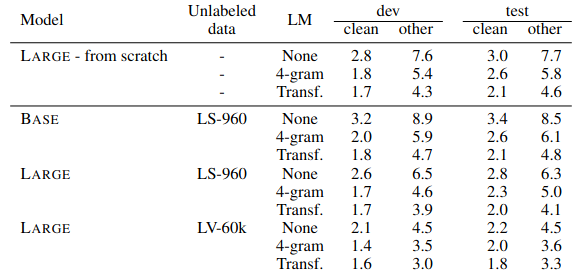
\includegraphics[width=1\textwidth]{boost-results.png}
    \caption{Rezultatele obținute cu un model simplu, un model de limbaj bazat pe n-grame și un model de limbaj bazat pe Transformer}
    \label{fig:boost-results}
\end{figure}

\par
Deoarece modelul de limbaj bazat pe \textit{Transformer} necesită considerabil mai mult timp pentru antrenare și inferență,
iar îmbunătățirea pe care o aduce nu este cu mult mai semnificativă decât cea adusă de un model de limbaj
bazat pe n-grame, am ales să folosesc doar modelul îmbunătățit cu n-grame.

\section{Clasificarea videoclipurilor}
\label{sec:clasificare-videoclipuri}
Videoclipurile încărcate pe platform vin însoțite de metadate precum: titlu, descriere și, folosind
modelul prezentat anterior, subtitrări. Pentru o experiență mai personalizată, am ales să clasific
videoclipurile în funcție de subiectul abordat în topicuri precum: politică, sport, divertisment,
tehnologie și afaceri. Am folosit un modelul de clasificare \textbf{BERT} (Bidirectional Encoder Representations
from Transformers) dezvoltat de \textit{Google} \cite{devlin2019bert} pe care l-am antrenat pe setul de date
\textit{BBC News} \cite{greene06icml}.

\subsection{Arhitectura modelului}
Modelul \textit{BERT} este un model de învățare profundă care are la bază partea de encodare a unui \textit{Transformer} \cite{vaswani2023attention},
scopul lui fiind de a înțelege contextul cuvintelor într-o propoziție. Modelul \textit{BERT} vine în două
variante: \textit{BERT-base} și \textit{BERT-large}, cele două diferă prin numărul de blocuri de encodare (12 și 24),
numărul de neuroni din stratul pentru clasificare (\textit{fully-connected}) (768 și 1024) și numărul de
capete de atenție (\textit{attention heads}) (12 și 16).

\par
Spre deosebire de arhitectura standard a unui \textit{Transformer}, \textit{BERT} adaugă un token
special la începutul fiecărei propoziții, \textit{[CLS]}, folosit pentru clasificare. Intuitiv,
acest token va reține informații despre întreaga propoziție și va putea fi folosit pentru rețeaua
de clasificare care va determina topicul propoziției. \ref{fig:bert-architecture}

\begin{figure}[h]
    \centering
    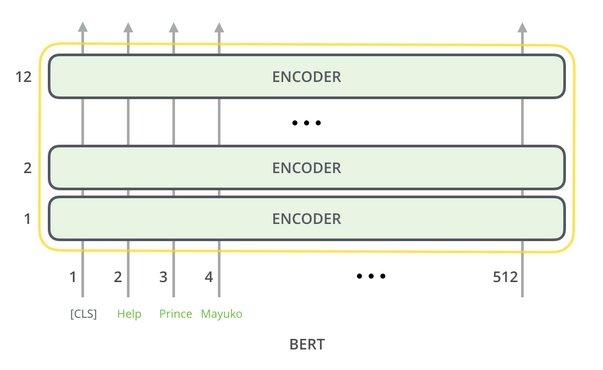
\includegraphics[width=1\textwidth]{bert-architecture.png}
    \caption{Arhitectura modelului \textit{BERT} \protect\footnotemark[2]}
    \label{fig:bert-architecture}
\end{figure}
\vspace{1em}

\par
Ieșirile modelului \textit{BERT} au dimensiunea 768, iar pentru partea de clasificare sunt trecute
prin un strat liniar (\textit{fully-connected}) cu 5 neuroni, câte unul pentru fiecare clasă.
Cu ajutorul funcției \textit{softmax}, se obține o distribuție de probabilitate peste cele
5 clase, iar clasa cu cea mai mare probabilitate este cea aleasă.

\footnotetext[2]{Imaginea a fost preluată de pe site-ul lui Jay Alammar, ``The Illustrated BERT, ELMo, and co. (How NLP Cracked Transfer Learning)'', disponibil la: \url{https://jalammar.github.io/illustrated-bert/}.}

\vspace{1em}

\subsection{Setul de date}
\vspace{1em}
Pentru antrenarea modelului am folosit setul de date \textit{BBC News} care conține 2225 de articole 
între anii 2004-2005. Setul de date este împărțit în 5 clase: politică, sport, divertisment, tehnologie
și afaceri. Mai jos am prezentat distribuția datelor din setul de date din punct de vedere al exemplelor
pe clasă și al lungimii medii a articolelor. \ref{fig:bbc-stats}

\vspace{1em}

\begin{figure}[h]
    \centering
    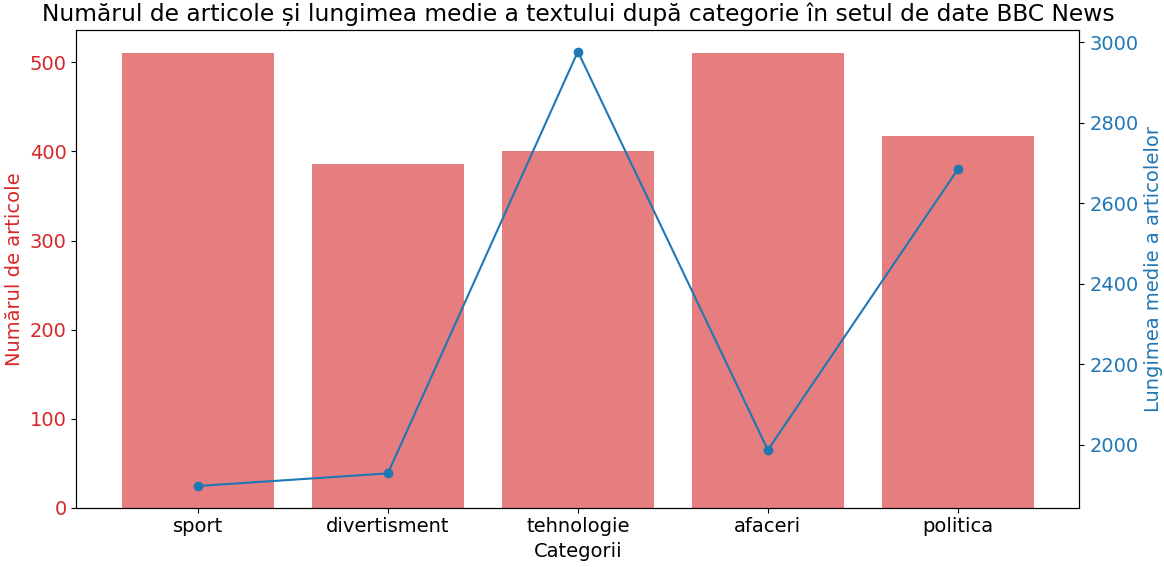
\includegraphics[width=0.9\textwidth]{bbc_stats_ro.png}
    \caption{Distribuția claselor din setul de date \textit{BBC News}}
    \label{fig:bbc-stats}
\end{figure}

\vspace{-0.5em}
\subsection{Antrenarea modelului}
\vspace{1em}
Antrenarea modelului a fost făcută folosind limbajul de programare Python, biblioteca PyTorch \cite{paszke2019pytorch}
și plecând de la modelul preantrenat \textit{bert-base-uncased} pus la dispoziție de Hugging Face.
Codul a fost structurat în: 
\vspace{1em}

\begin{itemize}
    \item \textbf{dataset.py} - creează un Dataset specific PyTorch pentru setul de date \textit{BBC News},
    implementând metodele \textit{\_\_len\_\_} și \textit{\_\_getitem\_\_}; metoda \textit{\_\_getitem\_\_}
    aplică tokenizer-ul pe text cu lungimea maximă de 512 token-uri și returnează un tuplu de \textit{input\_ids},
    \textit{attention\_mask} și \textit{label}.
    \item \textbf{model.py} - definește arhitectura modelului \textit{BERT} și a rețelei de clasificare:
    inițializează modelul preantrenat \textit{bert-base-uncased}, extrage token-ul special \textit{[CLS]}
    și adaugă un strat liniar cu 5 neuroni pentru clasificare.
    \item \textbf{trainer.py} - antrenează modelul pe setul de date \textit{BBC News} folosind
    hiperparametrii primiți din linia de comandă și salvează modelul de fiecare dată când obține o
    acuratețe mai bună pe setul de validare.
\end{itemize}


\par
În figurile de mai jos \ref{fig:loss_graphs} sunt ilustrate pierderile de antrenare și de evaluare pentru modelul \textit{BERT}
folosind ca rată de învățare $1 \times 10^{-4}$ și $1 \times 10^{-5}$. Se observă fenomenul de \textit{overfitting}
pentru rata de învățare $1 \times 10^{-4}$, motiv pentru care am ales să experimentez cu valori mai mici.

\begin{figure}[ht]
    \centering
    \begin{subfigure}[b]{0.49\textwidth}
        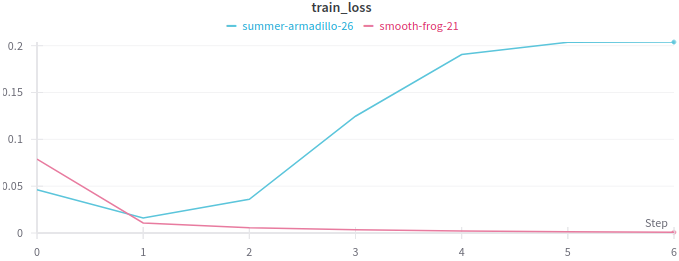
\includegraphics[width=1\textwidth]{train_loss_1.png}
        \caption{Pierdere de antrenare}
        \label{fig:train_loss}
    \end{subfigure}
    \hfill % Asigură spațierea dintre subfiguri
    \begin{subfigure}[b]{0.49\textwidth}
        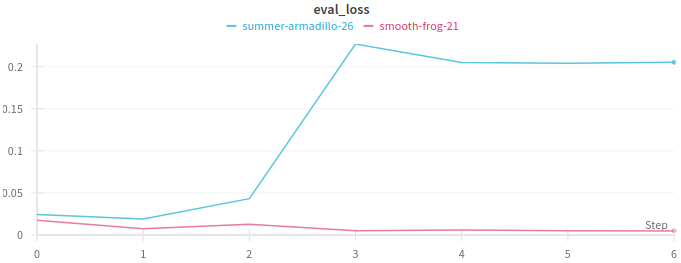
\includegraphics[width=1\textwidth]{eval_loss_1.png}
        \caption{Pierdere de validare}
        \label{fig:eval_loss}
    \end{subfigure}
    \caption{Pierderile de antrenare și de validare pentru modelul \textit{BERT}}
    \label{fig:loss_graphs}
\end{figure}
\vspace{-1em}

\par
Am încercat mai multe experimente plecând de la aceeași hiperparametri, cu rata de învățare $1 \times 10^{-5}$,
pentru a vedea cum e comportă modelul la diferite inițializări ale ponderilor. În figura \ref{fig:eval_acc}
se observă că acuratețile obținute sunt în intervalul 0.95-0.99. Am ales, în final, să folosesc modelul
cu cele mai mari valori obținute pe setul de validare.

\begin{figure}[h]
    \centering
    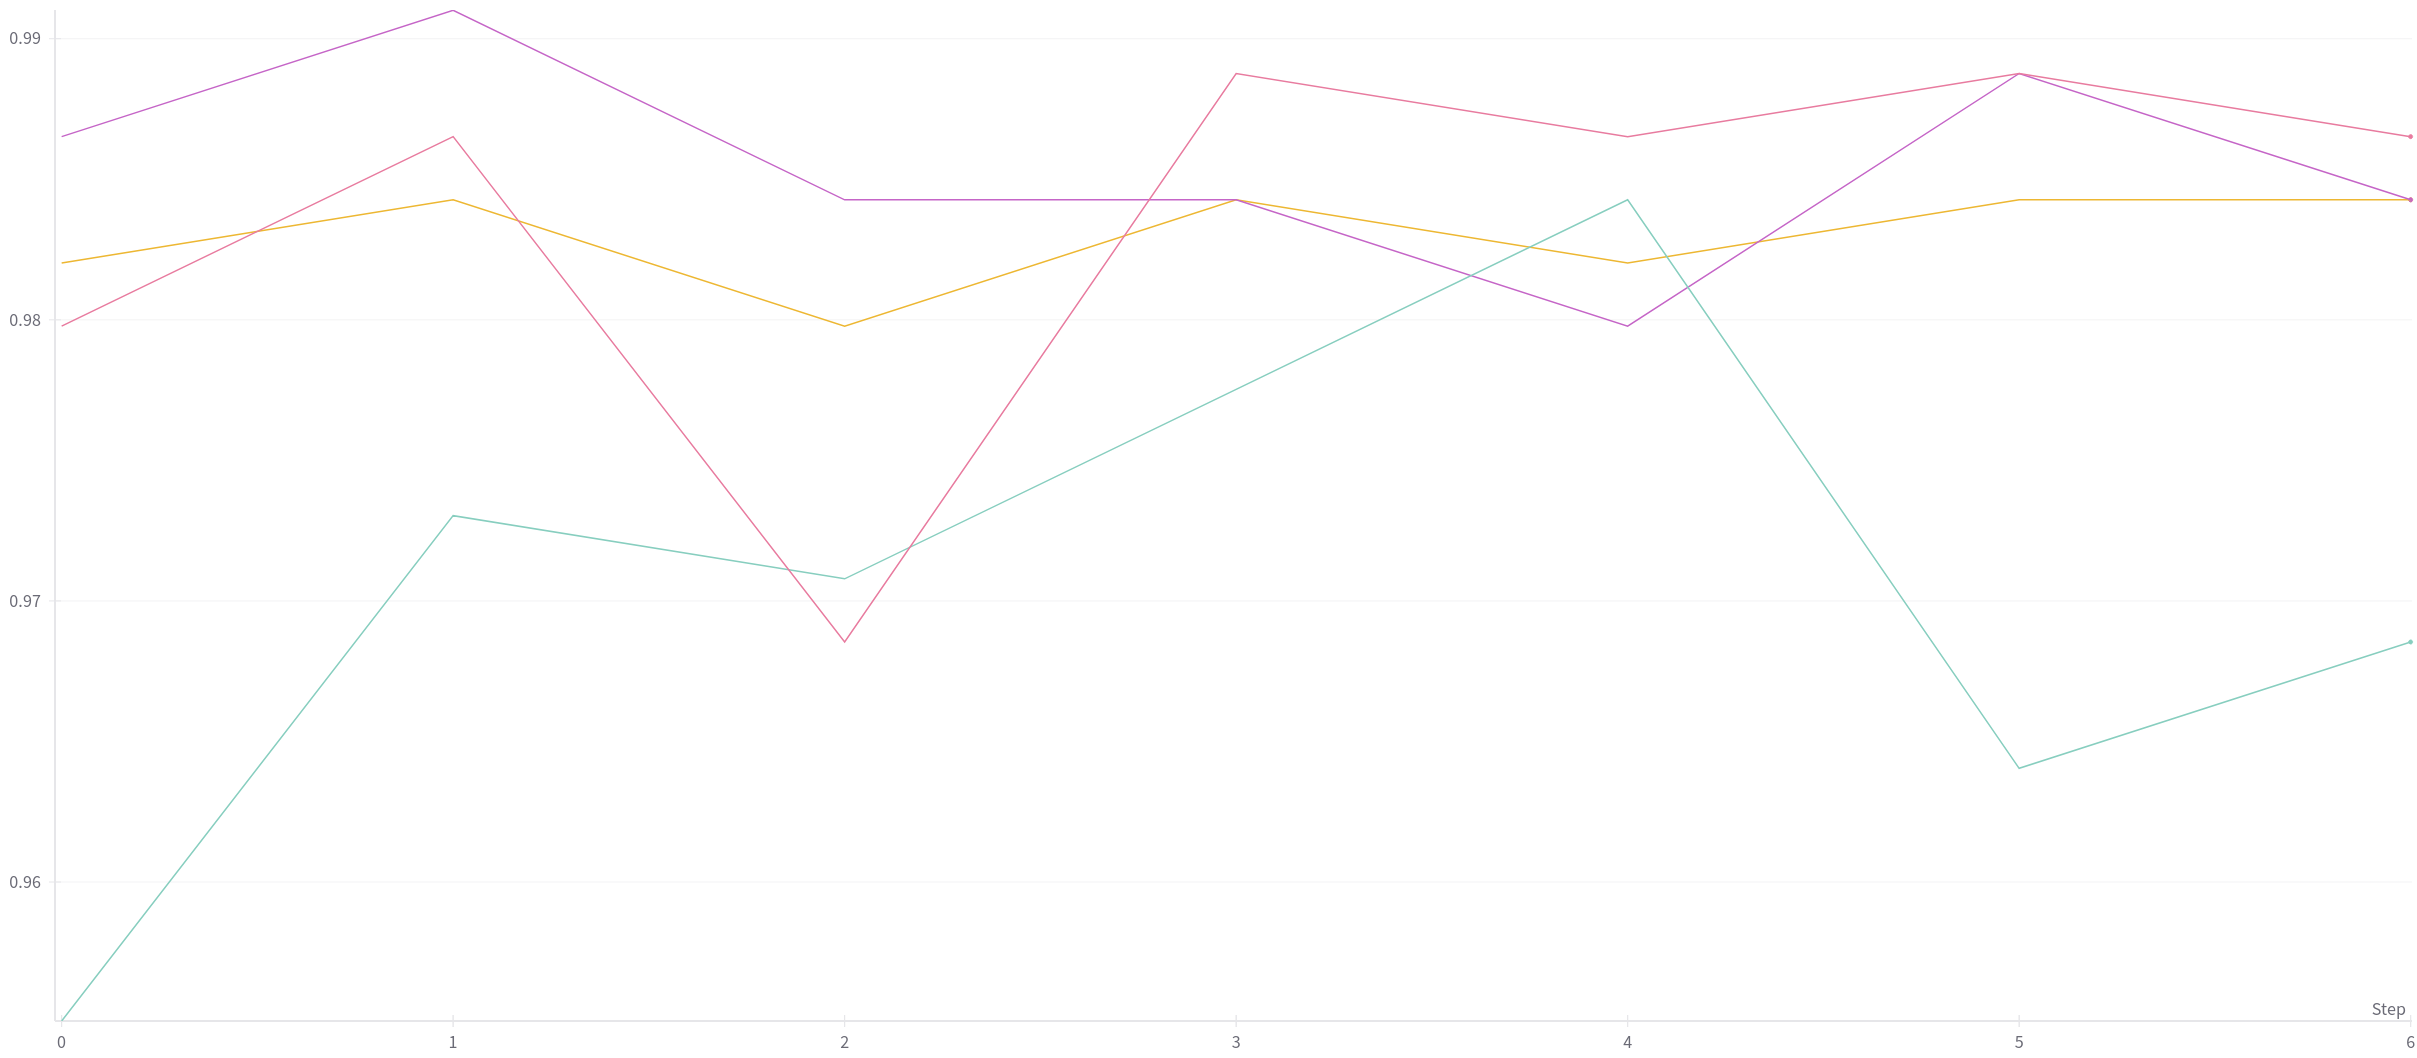
\includegraphics[width=0.8\textwidth]{eval_acc.png}
    \caption{Antrenamentele modelului \textit{BERT} cu rata de învățare $1 \times 10^{-5}$}
    \label{fig:eval_acc}
\end{figure}

\vspace{-1.5em}
\subsubsection{Hiperparametrii}
Pentru modelul final pe care l-am folosit pentru clasificarea videoclipurilor am ales următorii hiperparametrii:

% \begin{table}[h]
%     \centering
%     \label{tab:wav2vec2-hyperparameters}
%     \begin{tabular}{ll}
%     \hline
%     \textbf{Hiperparametru} & \textbf{Valoare} \\ \hline
%     Rata de învățare (\textit{learning rate}) & $1 \times 10^{-4}$ \\
%     Descreșterea greutății (\textit{weight decay}) & 0.005 \\
%     Pași de încălzire (\textit{warmup steps}) & 1000 \\
%     Dimensiunea lotului (\textit{batch size}) & 4 \\ \hline
%     \end{tabular}
%     \caption{Hiperparametrii folosiți pentru fine-tuning-ul modelului \textit{wav2vec2}}
% \end{table}

\begin{table}[ht]
    \centering
    \begin{tabular}{@{}ll@{}}
        \toprule
        \textbf{Hiperparametru}   & \textbf{Valoare}         \\
        \midrule
        Rată de învățare             & 0.00001                  \\
        Dimensiunea lotului             & 8                        \\
        Optimizator                      & Adam                     \\
        Funcția de pierdere          & CrossEntropyLoss         \\
        \bottomrule
    \end{tabular}
    \caption{Hiperparametrii modelului \textit{BERT}}
    \label{tab:bert-hyperparameters}
\end{table}


\subsection{Îmbunătățirea clasificării}
Videoclipurile pe care le vom clasifica mai departe conțin informații precum: titlu, descriere și subtitrări.
O primă observație este că titlul și descrierea sunt de obicei scurte și se poate deduce topicul videoclipului
doar din aceste două informații. Subtitrările, pe de altă parte, sunt mai lungi și conțin mai multe informații 
irelevante pentru clasificare. 
\par
În acest sens, textul alcătuit din titlu, descriere și subtitrări va fi împărțit în blocuri de căte 512 token-uri
pentru a respecta restricția de intrare a modelului \textit{BERT}. Pentru a exploata observația de mai sus,
vom folosi doar primele 10 blocuri de text pentru a clasifica videoclipul și vom da o importanță mai mare în
votul final primului bloc de text, care conține titlul și descrierea videoclipului.
\par
Pentru rezultatul final, vom alege topicul cu frecevența majoritară din cele 10 blocuri de text.


\section{Concluzie}
Cele două modele prezentate anterior, \textit{wav2vec 2.0} și \textit{BERT}, au fost încărcate
pe platforma \textit{Hugging Face} și sunt disponibile în pachetul \textit{transformers}.

\subsubsection{wav2vec 2.0}
Utilizarea modelului de recunoaștere a vorbirii necesită folosirea modulului \textit{Wav2Vec2ForCTC}
și a modulului \textit{Wav2Vec2Processor}, respectiv \textit{Wav2Vec2ProcessorWithLM} pentru a folosi varianta
îmbunătățită cu n-grame. Modelele se găsesc pe \textit{Hugging Face} și se pot accesa din pachetul \textit{transformers} astfel:

\begin{itemize}
    \item \textit{Mini LibriSpeech} - \textit{3funnn/wav2vec2-base-minilibrispeech}, respectiv \textit{3funnn/wav2vec2-base-minilibrispeech-lm} 
    pentru modelul îmbunătățit cu n-grame
    \item \textit{Common Voice Delta Segment 16.1} - \textit{3funnn/wav2vec2-base-common-voice}, respectiv \textit{3funnn/wav2vec2-base-common-voice-lm}
    pentru modelul îmbunătățit cu n-grame
\end{itemize}

\subsubsection{BERT}
Modelul de clasificare a videoclipurilor este disponibil în pachetul \textit{transformers} sub numele
\textit{3funnn/bert-topic-classification}. Modelul primește ca intrare un text (care poate fi o 
concatenare a titlului și a descrierii videoclipului) și returnează o distribuție de probabilitate
pentru fiecare din cele 5 clase. \textit{Hugging Face} pune la dispoziție funcția \textit{pipeline} care
permite folosirea modelului într-un mod simplu.
